\documentclass[14pt]{article}

\usepackage[english]{babel}
\usepackage{geometry}
\usepackage{graphicx}
\usepackage{float}
\usepackage{extsizes}
\usepackage{blindtext}
\usepackage{hyperref}

\geometry{
 a4paper,
 total={170mm,257mm},
 left=20mm,
 top=20mm,
 }
\graphicspath{ {../res/} }
\hypersetup{
    colorlinks = false,
    pdftitle = {Dwarf Guide},
    pdfpagemode=FullScreen,
}

\title{Dwarf Guide}
\author{h4nto}

\begin{document}

% FIRST PAGE:

\topskip0pt
\begin{center}
    \vspace*{\fill}
    \Huge\textbf{Dwarf Guide} \\
    \begin{figure}[h]
        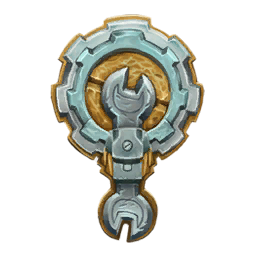
\includegraphics{dwarf.png}
        \centering
    \end{figure}
    \vspace*{\fill}
    \normalsize{A detailed Steam Mechanicus guide to help beginners,\\mid game and end game players and pvp players.} \\
    \vspace*{\fill}
    \Large\textsl{Written by h4nto} \\
    \Large\textsl{h4nto\#6969}
    \vspace*{\fill}
\end{center}

\newpage

% INDEX:

\tableofcontents

\newpage

\section{Beginners}

\subsection{Wisdom}
Talking about Wisdom, the first things to focus on are Attack Speed (put there points until you reach 4.00 Attack Speed, so you will get the damage buff in map) and most of all Critical (to max 80/80 as soon as possible).
After that you can start using your points on what you think you need at that moment.
Generally it's defensive stats such as HP, Armor and Resistances or eventually some Steam if you feel you run out of resources too quickly.

\subsection{Group Tree}

\subsection{Gems}
Talking about Gems, as always Critical is the most important thing, try to have a balanced build but most of all work to get the 4.00 Attack Speed and upgrade your Critical gems as much as possible.
Other Gems to equip are Movement Speed, Damage and HP.

\subsection{Runes}
Talking about Runes, first of all you should work on your Wisdom and Materi runes (upgrade them as much as possible because they will allow you to level up your Wisdom way faster and also get faster the Materi to buy Infernal Passages).
After them again focus first on Attack Speed and Critical. Then go for HP, Damage and Movement Speed but don't throw away Steam and Steam Regeneration ones, equip them and upgrade them later.
Another Rune that is particularly good is Realm Fragment Talent Rune (you will need to max that in order to join groups for Realm Fragments farm) together with Wisdom and Andermants Talent Runes.
Every other kind of Rune you can melt for now.

\subsection{Jewels}

\subsection{Items}

\subsection{Build}

\subsubsection{build 1}

\subsubsection{build 2}

\subsubsection{build 3}

\subsection{Skilltree}


\newpage

\section{Mid Game}
\subsection{Wisdom}
\subsection{Gems}
\subsection{Runes}
\subsection{Jewels}
\subsection{Items}
\subsection{Build}
\subsubsection{build 1}
\subsubsection{build 2}
\subsubsection{build 3}
\subsection{Skilltree}

\newpage

\section{End Game}
\subsection{Wisdom}
\subsection{Gems}
\subsection{Runes}
\subsection{Jewels}
\subsection{Items}
\subsection{Build}
\subsubsection{build 1}
\subsubsection{build 2}
\subsubsection{build 3}
\subsection{Skilltree}

\newpage

\section{PvP}
\subsection{PvP Tree}
\subsection{Gems}
\subsection{Items}
\subsection{Build}
\subsubsection{build 1}
\subsubsection{build 2}
\subsubsection{build 3}
\subsection{Skilltree}

\newpage

\end{document}